%% pscc2022_template.tex, V1.1, 2019/03/11
%% by Mario Paolone
%% This is a Latex template to prepare submissions for the PSCC 2022 conference. 
%% The template demonstrates the use of the class IEEEtran4PSCC.cls and is mostly
%% based on the file bare_conf.tex (V1.4a) by Michael Shell.

%%*************************************************************************
%% Legal Notice:
%% This code is offered as-is without any warranty either expressed or
%% implied; without even the implied warranty of MERCHANTABILITY or
%% FITNESS FOR A PARTICULAR PURPOSE! 
%% User assumes all risk.
%% In no event shall PSCC or any contributor to this code be liable for
%% any damages or losses, including, but not limited to, incidental,
%% consequential, or any other damages, resulting from the use or misuse
%% of any information contained here.
%%
%% All comments are the opinions of their respective authors and are not
%% necessarily endorsed by the PSCC.
%%
%% This work is distributed under the LaTeX Project Public License (LPPL)
%% ( http://www.Latex-project.org/ ) version 1.3, and may be freely used,
%% distributed and modified. A copy of the LPPL, version 1.3, is included
%% in the base LaTeX documentation of all distributions of LaTeX released
%% 2003/12/01 or later.
%% Retain all contribution notices and credits.
%% ** Modified files should be clearly indicated as such, including  **
%% ** renaming them and changing author support contact information. **
%%
%% File list of work: pscc2022_template.tex, IEEEtran4PSCC.cls
%%*************************************************************************


% *** Authors should verify (and, if needed, correct) their LaTeX system  ***
% *** with the testflow diagnostic prior to trusting their LaTeX platform ***
% *** with production work.                 ***


\documentclass{IEEEtran4PSCC}
% The automatically selected options are the format (US letter) and conference mode.


% Some very useful LaTeX packages include:
% (uncomment the ones you want to load)
% *** MISC UTILITY PACKAGES ***
%
%\usepackage{ifpdf}
% Heiko Oberdiek's ifpdf.sty is very useful if you need conditional
% compilation based on whether the output is pdf or dvi.
% usage:
% \ifpdf
%   % pdf code
% \else
%   % dvi code
% \fi
% The latest version of ifpdf.sty can be obtained from:
% http://www.ctan.org/tex-archive/macros/Latex/contrib/oberdiek/
% Also, note that IEEEtran.cls V1.7 and later provides a builtin
% \ifCLASSINFOpdf conditional that works the same way.
% When switching from Latex to pdfLatex and vice-versa, the compiler may
% have to be run twice to clear warning/error messages.

% *** CITATION PACKAGES ***
%
%\usepackage{cite}
% cite.sty was written by Donald Arseneau
% V1.6 and later of IEEEtran pre-defines the format of the cite.sty package
% \cite{} output to follow that of IEEE. Loading the cite package will
% result in citation numbers being automatically sorted and properly
% 'compressed/ranged'. e.g., [1], [9], [2], [7], [5], [6] without using
% cite.sty will become [1], [2], [5]--[7], [9] using cite.sty. cite.sty's
% \cite will automatically add leading space, if needed. Use cite.sty's
% noadjust option (cite.sty V3.8 and later) if you want to turn this off
% such as if a citation ever needs to be enclosed in parenthesis.
% cite.sty is already installed on most LaTeX systems. Be sure and use
% version 5.0 (2009-03-20) and later if using hyperref.sty.
% The latest version can be obtained at:
% http://www.ctan.org/tex-archive/macros/Latex/contrib/cite/
% The documentation is contained in the cite.sty file itself.


% *** GRAPHICS RELATED PACKAGES ***
%
\ifCLASSINFOpdf
   \usepackage[pdftex]{graphicx}
  % declare the path(s) where your graphic files are
  % \graphicspath{{../pdf/}{../jpeg/}}
  % and their extensions so you won't have to specify these with
  % every instance of \includegraphics
  % \DeclareGraphicsExtensions{.pdf,.jpeg,.png}
\else
  % or other class option (dvipsone, dvipdf, if not using dvips). graphicx
  % will default to the driver specified in the system graphics.cfg if no
  % driver is specified.
   \usepackage[dvips]{graphicx}
  % declare the path(s) where your graphic files are
  % \graphicspath{{../eps/}}
  % and their extensions so you won't have to specify these with
  % every instance of \includegraphics
  % \DeclareGraphicsExtensions{.eps}
\fi
% graphicx was written by David Carlisle and Sebastian Rahtz. It is
% required if you want graphics, photos, etc. graphicx.sty is already
% installed on most LaTeX systems. The latest version and documentation
% can be obtained at: 
% http://www.ctan.org/tex-archive/macros/Latex/required/graphics/
% Another good source of documentation is 'Using Imported Graphics in
% LaTeX2e' by Keith Reckdahl which can be found at:
% http://www.ctan.org/tex-archive/info/epsLatex/
%
% Latex, and pdfLatex in dvi mode, support graphics in encapsulated
% postscript (.eps) format. pdfLatex in pdf mode supports graphics
% in .pdf, .jpeg, .png and .mps (metapost) formats. Users should ensure
% that all non-photo figures use a vector format (.eps, .pdf, .mps) and
% not a bitmapped formats (.jpeg, .png). IEEE frowns on bitmapped formats
% which can result in 'jaggedy'/blurry rendering of lines and letters as
% well as large increases in file sizes.
%
% You can find documentation about the pdfTeX application at:
% http://www.tug.org/applications/pdftex



% *** MATH PACKAGES ***
%
\usepackage[cmex10]{amsmath}
\usepackage{xcolor}
% A popular package from the American Mathematical Society that provides
% many useful and powerful commands for dealing with mathematics. If using
% it, be sure to load this package with the cmex10 option to ensure that
% only type 1 fonts will utilized at all point sizes. Without this option,
% it is possible that some math symbols, particularly those within
% footnotes, will be rendered in bitmap form which will result in a
% document that can not be IEEE Xplore compliant!
%
% Also, note that the amsmath package sets \interdisplaylinepenalty to 10000
% thus preventing page breaks from occurring within multiline equations. Use:
%\interdisplaylinepenalty=2500
% after loading amsmath to restore such page breaks as IEEEtran.cls normally
% does. amsmath.sty is already installed on most LaTeX systems. The latest
% version and documentation can be obtained at:
% http://www.ctan.org/tex-archive/macros/Latex/required/amsLatex/math/





% *** SPECIALIZED LIST PACKAGES ***
%
% \usepackage{algorithmic}
% algorithmic.sty was written by Peter Williams and Rogerio Brito.
% This package provides an algorithmic environment fo describing algorithms.
% You can use the algorithmic environment in-text or within a figure
% environment to provide for a floating algorithm. Do NOT use the algorithm
% floating environment provided by algorithm.sty (by the same authors) or
% algorithm2e.sty (by Christophe Fiorio) as IEEE does not use dedicated
% algorithm float types and packages that provide these will not provide
% correct IEEE style captions. The latest version and documentation of
% algorithmic.sty can be obtained at:
% http://www.ctan.org/tex-archive/macros/Latex/contrib/algorithms/
% There is also a support site at:
% http://algorithms.berlios.de/index.html
% Also of interest may be the (relatively newer and more customizable)
% algorithmicx.sty package by Szasz Janos:
% http://www.ctan.org/tex-archive/macros/Latex/contrib/algorithmicx/




% *** ALIGNMENT PACKAGES ***
%
%\usepackage{array}
% Frank Mittelbach's and David Carlisle's array.sty patches and improves
% the standard LaTeX2e array and tabular environments to provide better
% appearance and additional user controls. As the default LaTeX2e table
% generation code is lacking to the point of almost being broken with
% respect to the quality of the end results, all users are strongly
% advised to use an enhanced (at the very least that provided by array.sty)
% set of table tools. array.sty is already installed on most systems. The
% latest version and documentation can be obtained at:
% http://www.ctan.org/tex-archive/macros/Latex/required/tools/


% IEEEtran contains the IEEEeqnarray family of commands that can be used to
% generate multiline equations as well as matrices, tables, etc., of high
% quality.




% *** SUBFIGURE PACKAGES ***
%\ifCLASSOPTIONcompsoc
%  \usepackage[caption=false,font=normalsize,labelfont=sf,textfont=sf]{subfig}
%\else
%  \usepackage[caption=false,font=footnotesize]{subfig}
%\fi
% subfig.sty, written by Steven Douglas Cochran, is the modern replacement
% for subfigure.sty, the latter of which is no longer maintained and is
% incompatible with some LaTeX packages including fixltx2e. However,
% subfig.sty requires and automatically loads Axel Sommerfeldt's caption.sty
% which will override IEEEtran.cls' handling of captions and this will result
% in non-IEEE style figure/table captions. To prevent this problem, be sure
% and invoke subfig.sty's 'caption=false' package option (available since
% subfig.sty version 1.3, 2005/06/28) as this is will preserve IEEEtran.cls
% handling of captions.
% Note that the Computer Society format requires a larger sans serif font
% than the serif footnote size font used in traditional IEEE formatting
% and thus the need to invoke different subfig.sty package options depending
% on whether compsoc mode has been enabled.
%
% The latest version and documentation of subfig.sty can be obtained at:
% http://www.ctan.org/tex-archive/macros/Latex/contrib/subfig/




% *** FLOAT PACKAGES ***
%
%\usepackage{fixltx2e}
% fixltx2e, the successor to the earlier fix2col.sty, was written by
% Frank Mittelbach and David Carlisle. This package corrects a few problems
% in the LaTeX2e kernel, the most notable of which is that in current
% LaTeX2e releases, the ordering of single and double column floats is not
% guaranteed to be preserved. Thus, an unpatched LaTeX2e can allow a
% single column figure to be placed prior to an earlier double column
% figure. The latest version and documentation can be found at:
% http://www.ctan.org/tex-archive/macros/Latex/base/


%\usepackage{stfloats}
% stfloats.sty was written by Sigitas Tolusis. This package gives LaTeX2e
% the ability to do double column floats at the bottom of the page as well
% as the top. (e.g., '\begin{figure*}[!b]' is not normally possible in
% LaTeX2e). It also provides a command:
%\fnbelowfloat
% to enable the placement of footnotes below bottom floats (the standard
% LaTeX2e kernel puts them above bottom floats). This is an invasive package
% which rewrites many portions of the LaTeX2e float routines. It may not work
% with other packages that modify the LaTeX2e float routines. The latest
% version and documentation can be obtained at:
% http://www.ctan.org/tex-archive/macros/Latex/contrib/sttools/
% Do not use the stfloats baselinefloat ability as IEEE does not allow
% \baselineskip to stretch. Authors submitting work to the IEEE should note
% that IEEE rarely uses double column equations and that authors should try
% to avoid such use. Do not be tempted to use the cuted.sty or midfloat.sty
% packages (also by Sigitas Tolusis) as IEEE does not format its papers in
% such ways.
% Do not attempt to use stfloats with fixltx2e as they are incompatible.
% Instead, use Morten Hogholm'a dblfloatfix which combines the features
% of both fixltx2e and stfloats:
%
% \usepackage{dblfloatfix}
% The latest version can be found at:
% http://www.ctan.org/tex-archive/macros/Latex/contrib/dblfloatfix/




% *** PDF, URL AND HYPERLINK PACKAGES ***
%
% \usepackage{url}
% url.sty was written by Donald Arseneau. It provides better support for
% handling and breaking URLs. url.sty is already installed on most LaTeX
% systems. The latest version and documentation can be obtained at:
% http://www.ctan.org/tex-archive/macros/Latex/contrib/url/
% Basically, \url{my_url_here}.




% *** Do not adjust lengths that control margins, column widths, etc. ***
% *** Do not use packages that alter fonts (such as psLatex).         ***
% There should be no need to do such things with IEEEtran.cls V1.6 and later.


% correct bad hyphenation here
\hyphenation{op-tical net-works semi-conduc-tor}
\usepackage[bookmarks=false]{hyperref}
\usepackage{amsmath}
\usepackage{stfloats}

% Set footer
\makeatletter
\let\old@ps@headings\ps@headings
\let\old@ps@IEEEtitlepagestyle\ps@IEEEtitlepagestyle
\def\psccfooter#1{%
    \def\ps@headings{%
        \old@ps@headings%
        \def\@oddfoot{\strut\hfill#1\hfill\strut}%
        \def\@evenfoot{\strut\hfill#1\hfill\strut}%
    }%
    \def\ps@IEEEtitlepagestyle{%
        \old@ps@IEEEtitlepagestyle%
        \def\@oddfoot{\strut\hfill#1\hfill\strut}%
        \def\@evenfoot{\strut\hfill#1\hfill\strut}%
    }%
    \ps@headings%
}
\makeatother

\psccfooter{%
        \parbox{\textwidth}{\hrulefill \\ \small{22nd Power Systems Computation Conference} \hfill \begin{minipage}{0.2\textwidth}\centering \vspace*{4pt} 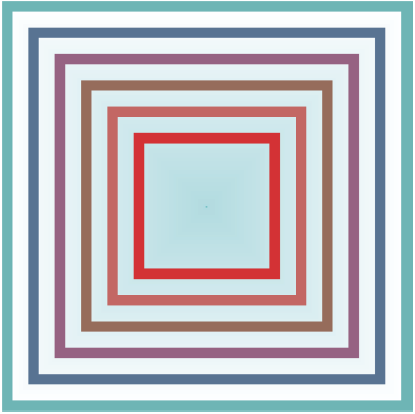
\includegraphics[scale=0.06]{PSCC_logo.png}\\\small{PSCC 2022} \end{minipage} \hfill \small{Porto, Portugal --- June 27 -- July 1, 2022}}%
}

\begin{document}
%
% paper title
% Titles are generally capitalized except for words such as a, an, and, as,
% at, but, by, for, in, nor, of, on, or, the, to and up, which are usually
% not capitalized unless they are the first or last word of the title.
% Linebreaks \\ can be used within to get better formatting as desired.
% Do not put math or special symbols in the title.
\title{Total AC Interferences Between a Power Line Subject to a Single-Phase Fault and a Nearby Pipeline with Multilayered Soil}


%% To specify the authors when (number of affiliations <= 2)
\author{
\IEEEauthorblockN{Caio M. Moraes\\ Gustavo H. de Sá Matos \IEEEauthorrefmark{1}\\ Amauri G. Martins-Britto \\ Kleber M. Silva}
\IEEEauthorblockA{Department of Electrical Engineering \\
University of Brasília, UnB\\
Brasília, Brazil\\
\{caiomoraes@lapse., amaurigm@, klebermelo@\}unb.br, gustavodesamatos@gmail.com\IEEEauthorrefmark{1}}
}


%% To specify the authors when (number of affiliations > 2)
% \author{\IEEEauthorblockN{Author n.1\IEEEauthorrefmark{1},
% Author n.2\IEEEauthorrefmark{2},
% Author n.3\IEEEauthorrefmark{3}, 
% Author n.4\IEEEauthorrefmark{3} and
% Author n.5\IEEEauthorrefmark{4}}
% \IEEEauthorblockA{\IEEEauthorrefmark{1} Department Name of Organization A\\
% Name of the organization A,
% Address A\\ Emails if wanted}
% \IEEEauthorblockA{\IEEEauthorrefmark{2} Department Name of Organization B\\
% Name of the organization B,
% Address B\\ Emails if wanted}
% \IEEEauthorblockA{\IEEEauthorrefmark{3} Department Name of Organization C\\
% Name of the organization C,
% Address C\\ Emails if wanted}
% \IEEEauthorblockA{\IEEEauthorrefmark{4}Department Name of Organization D\\
% Name of the organization D,
% Address D\\ Emails if wanted}
% }


% make the title area
\maketitle

% As a general rule, do not put math, special symbols or citations
% in the abstract
\begin{abstract}
This paper describes the problem of electromagnetic interferences between power lines and metallic structures, caused by inductive and conductive coupling mechanisms, and the main risks to which personnel and facilities are exposed. An EMTP-based implementation is proposed to predict induced voltage levels on a target circuit, due to interferences caused by overhead power lines under steady-state nominal load, as well as fault conditions, using generalized formulas to represent the N-layered soil. Results are tested by means of a case study of a real shared right-of-way project and comparisons with results obtained using industry-standard software. Results show that the proposed method is accurate, with errors smaller than 8\%. Stress voltage values in the interfered pipeline are the order of 50 kV, exposing the structure  coating to risk of breakdown, which may lead to corrosion and pipeline failure. A mitigation is designed and proven to reduce voltage values to safe levels, in compliance with the nominal limits from the manufacturer.
\end{abstract}

\begin{IEEEkeywords}
Electromagnetic interferences, Electromagnetic Transient Program (EMTP), pipelines, single-phase fault and transmission lines.
\end{IEEEkeywords}


% Use this to place sponsorships
\thanksto{\noindent This work was developed  in partnership with IATI and CEPEL within the scope of the R\&D project PD-06908-0003/2021, sponsored by the Brazilian Agency of Electrical Energy (ANEEL) and EVOLTZ. The authors thank the cooperation of Ms. Larissa Silva (IATI) and Dr. Marco Antônio M. Rodrigues (CEPEL).}


\section{Introduction}


Overhead transmission lines (TLs) are large structures and
require large right-of-ways which often extend for several hundred kilometers. Due to the trend of sharing space with other facilities, forming the so called utility corridors, and the energy levels involved,  TLs may induce currents in nearby metal structures that are not designed to conduct electricity. This effect may raise risks to metallic installations neighboring the TLs through three types of electromagnetic interference (EMI) mechanisms: inductive, conductive and capacitive couplings \cite{CIGREWG36}.

EMIs are influenced by current levels flowing through TL conductors, length of exposure, soil characteristics and constructive aspects of the facilities involved \cite{CIGREWG36}. 

Serious design errors may occur if these EMI are not properly addressed, exposing personnel and installations to risks, which justifies the efforts in developing reliable and realistic simulation models.

EMI studies reported in the literature generally represent the soil as semi-infinite and homogeneous structure or represent N-layered soils by equivalent homogeneous models. This  approach is reported to yield inaccuracies in a variety of practical cases, due to the multilayered characteristic of natural soils  \cite{Qi2013,Wu2017,Alexandru2020}. Moreover, to the best of the author's knowledge, there is no report in the specialized EMI literature accounting for arbitrary multilayered soil models within the EMTP-based paradigm.

This paper presents an EMTP-based implementation for inductive and conductive coupling studies caused by a TL under nominal load and phase-to-ground fault conditions with multilayered soil models.

Self and mutual impedance calculations are based on a generalized solution for overhead and buried conductors considering N-layered soils, proposed by Tsimiatros et al \cite{Tsiamitros2008a}.

To properly account for earth conduction effects, the generalized N-layered Green's function, proposed by He et al. \cite{He2012} and Li et al. \cite{Li2006}, is used to represent the ground potential rise along the interfered structure, due to currents flowing into the soil under fault conditions.

The proposed implementation is leveraged to analyze the case of a real right-of-way in Brazil, shared between a 138 kV TL and an underground metallic pipeline. A 3-layered soil model is determined from local resistivity measurements. The proposed method is used to calculate the resulting stress voltages due to a phase-to-ground fault. 

The obtained results are compared with software CDEGS and present RMS errors of less than 8\% in the cases analyzed. Stress voltages in the pipeline coating yield values close to 50 kV, which subjects the installation to risks that must be addressed according to safety standards. 

Then, further simulations are performed to design a mitigation solution to reduce stress voltage levels along the interfered pipeline, which is demonstrated to reduce the initial stress voltage approximately in 50\%, thus ensuring compliance with industry standards.

\section{Mathematical Model}

\subsection{Inductive coupling}

Currents flowing in an energized conductor produces a time-varying magnetic field, as shown in Fig. \ref{fig:InductiveCoupling}. This time-varying magnetic field causes electromotive forces (EMFs) which, on their turn, induce voltages and currents on a metallic structure laid parallelly to the energized conductor. This electromagnetic phenomenon is known as inductive coupling \cite{CIGREWG36}.

The inductive influence of a transmission line conductor on a nearby pipeline depends on the current magnitude, distance between structures, exposure length, soil resistivity, as well as the characteristics of installations involved \cite{CIGREWG36}.

\begin{figure}[hbt]
	\begin{center}
		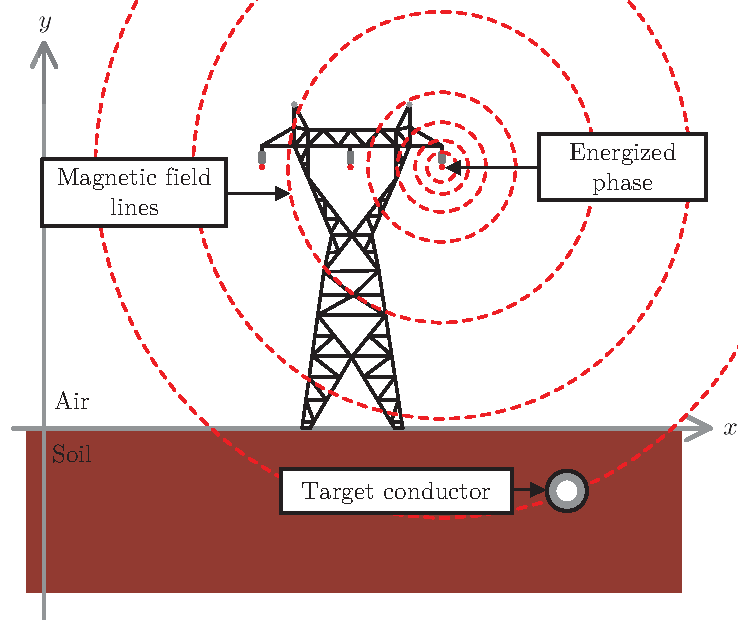
\includegraphics[width=1\columnwidth]{./fig/induc_coup2.pdf}
		\caption{Inductive coupling phenomenon, adapted from \cite{Martins-Britto2020}.}
		\label{fig:InductiveCoupling}
	\end{center}
\end{figure}

The induced EMF ($E$) is numerically given by \cite{CIGREWG36}:

\begin{equation}
		E = Z_{m} \times I
		\label{eq:emf_eq}
\end{equation}

\noindent in which $Z_{m}$ is the mutual impedance between the source and the target conductors, in ohms.meter; $I$ is the current in the energized conductor, in ampères; and $E$ is the EMF imposed to the target metallic structure, in volts per meter.

\subsection{Mutual impedance for N-layered soil}

\begin{figure*}[b]
	\hrulefill
	\begin{equation}\label{eq:Zij}
		\begin{aligned}
			Z_{i,j} = {} & \frac{j\omega\mu_{m}}{2\pi}\int_{0}^{\infty} \frac{cos(uy_{i,j})}{\bar\alpha_{m}} \times \left\{2^{m-l}\frac{(\mu_{1}\mu_{2}\dots\mu_{m-1})(\bar\alpha_{1}\bar\alpha_{2}\dots\bar\alpha_{m})(e^{-\bar\alpha_{l}d_{l}}e^{-\bar\alpha_{l+1}d_{l+1}}\dots e^{-\bar\alpha_{m}d_{m}})}{(\mu_{1}\mu_{2}\dots\mu_{l-1})(\bar\alpha_{1}\bar\alpha_{2}\dots\bar\alpha_{l})}\cdot\frac{\bar{F_{1}}\bar{F_{2}}}{D\bar{T}D_{0}}\right\}du,	\\
			\bar{F_{1}} = {} & [D\bar{T}D_{m} e^{\bar{\alpha}_{m}(d_{m}-h_{1})} + D\bar{T}N_{m}e^{-\bar{\alpha}_{m}(d_{m}-h_{1})}], \\			
			\bar{F_{2}} = {} & [T\bar{D}D_{l-1}e^{\bar{\alpha}_{1}h_{2}} + T\bar{D}N_{l-1}e^{-\bar{\alpha}_{1}h_{2}}].
		\end{aligned}
	\end{equation}
\end{figure*}


The mutual impedance, described by term $Z_{m}$ in \eqref{eq:emf_eq}, is calculated based on the generalized solution proposed by Tsiamitros et al. \cite{Tsiamitros2008a}, which extends the well-known Carson's \cite{Carson1926}, Nakagawa's \cite{Nakagawa} and Pollaczek's \cite{Pollaczek1926} original formulas and is reported to accurately handle complex configurations composed of both overhead and buried conductors in or above N-layered earth, as well as the displacement current effects, thus covering a frequency spectrum up to 1 MHz. 

Fig. \ref{fig:NlayeredSoil} illustrates two conductors $i$ and $j$ in an N-layered earth structure, in which each layer is described by the corresponding parameters permeability ($\mu_{i}$), permittivity ($\epsilon_{i}$), conductivity ($\sigma_{i}$) and thickness ($d_{i}$). Conductors are depicted as buried in the $m^{th}$ and $l^{th}$ layers of the N-layered earth, respectively, for illustration purposes, with no loss of generality. The per unit length mutual impedance $Z_m=Z_{i,j}$ is calculated from (\ref{eq:Zij}), in which $\omega = 2\pi f$ is the angular velocity, in radians per second; $h_{1}$ and $h_{2}$ are the relative vertical distances to the upper boundaries of layers $m$ and $l$, respectively, in meters; $y_{i,j}$ is the horizontal distance between  conductors $i$ and $j$, in meters; and $\bar{\alpha}_{i} = \sqrt{u^2 + \bar{\gamma}_{i}^{2}}$, $\bar{\gamma}_{i}^{2} = j\omega\mu_{i}(\sigma_{i} + j\omega\epsilon_{i})$, with $i = 0,1,2,\dots,N$ \cite{Tsiamitros2008a}.

\begin{figure}[hbt]
	\begin{center}
		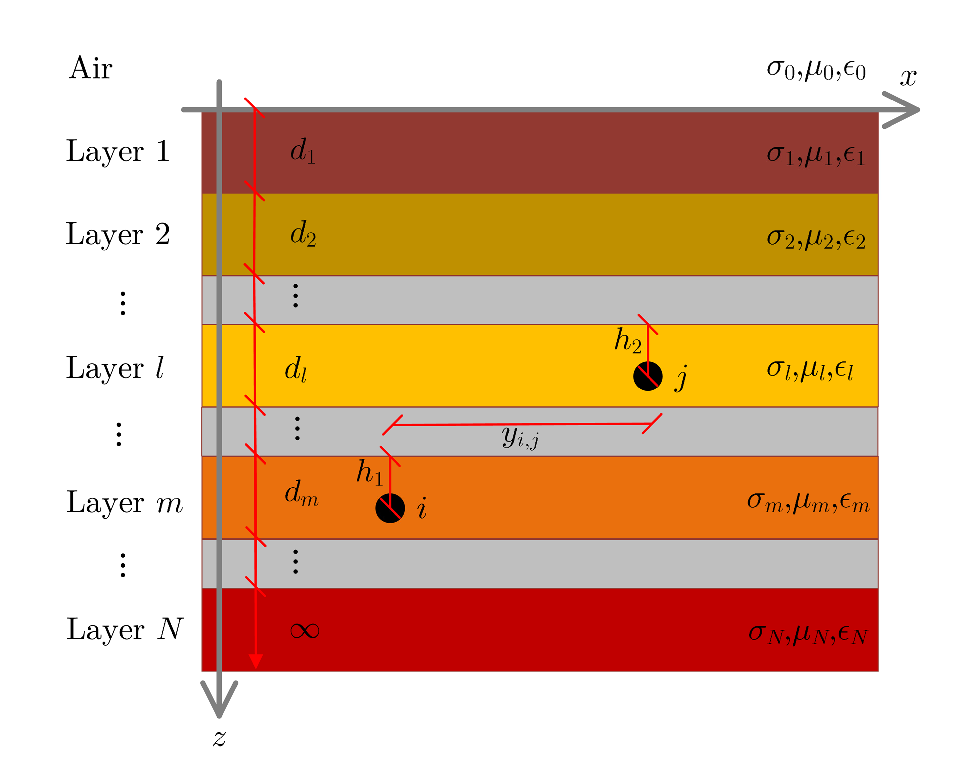
\includegraphics[width=1\columnwidth]{./fig/multilayered_soil2.pdf}
		\caption{Two underground conductors in N-layered soil.}
		\label{fig:NlayeredSoil}
	\end{center}
\end{figure}

Terms $D\bar{T}N_{i}$, $D\bar{T}D_{i}$, $T\bar{D}N_{k}$ and $T\bar{D}D_{k}$, given in (\ref{eq:DTN})-(\ref{eq:TDN}), relate the electromagnetic and geometric characteristics of the successive layers, in which $i = 0,1,2,\dots,N$ and $k = 0,1,2,\dots,m$. Following the same notation as \cite{Tsiamitros2008a}, the first characters of expressions TD (``Top to Down'') and DT (``Down to Top'') denote the direction of the recursive formulas, and the characters D (``Denominator'') and N (``Numerator'') indicate where each term usually appears during the formula expansion.

\begin{equation}\label{eq:DTN}
	\begin{aligned}
		D\bar{T}N_{i} = {} & (\mu_{i+1}\bar\alpha_{i} - \mu_{i}\bar\alpha_{i+1})D\bar{T}D_{i+1} \\
		& + (\mu_{i+1}\bar\alpha_{i} + \mu_{i}\bar\alpha_{i+1})D\bar{T}N_{i+1}e^{-2\bar\alpha_{i+1}d_{i+1}},
	\end{aligned}
\end{equation}  

\begin{equation}
	\begin{aligned}
		D\bar{T}D_{i} = {} & (\mu_{i+1}\bar\alpha_{i} + \mu_{i}\bar\alpha_{i+1})D\bar{T}D_{i+1} \\
		& + (\mu_{i+1}\bar\alpha_{i} - \mu_{i}\bar\alpha_{i+1})D\bar{T}N_{i+1}e^{-2\bar\alpha_{i+1}d_{i+1}},
	\end{aligned}
\end{equation} 

\begin{equation}
	D\bar{T}N_{N} = 0,
\end{equation}

\begin{equation}
	D\bar{T}D_{N} = 1,
\end{equation}

\begin{equation}
	T\bar{D}D_{-1} = 1,
\end{equation}

\begin{equation}
	T\bar{D}N_{-1} = 0,
\end{equation}

\begin{equation}
	\begin{aligned}
		T\bar{D}D_{k-1} = {} & (\mu_{k-1}\bar\alpha_{k} + \mu_{k}\bar\alpha_{k-1})T\bar{D}D_{k-2} \\
		& + (\mu_{k-1}\bar\alpha_{k} - \mu_{k}\bar\alpha_{k-1})T\bar{D}N_{k-2}e^{-2\bar\alpha_{k-1}d_{k-1}},
	\end{aligned}
\end{equation} 

\begin{equation}\label{eq:TDN}
	\begin{aligned}
		T\bar{D}N_{k-1} = {} & (\mu_{k-1}\bar\alpha_{k} - \mu_{k}\bar\alpha_{k-1})T\bar{D}D_{k-2} \\
		& + (\mu_{k-1}\bar\alpha_{k} + \mu_{k}\bar\alpha_{k-1})T\bar{D}N_{k-2}e^{-2\bar\alpha_{k-1}d_{k-1}}.
	\end{aligned}
\end{equation}




Coefficients described in (\ref{eq:DTN})-(\ref{eq:TDN}) define a recursive function dependent on the earth layer and positions of conductors $i$ and $j$, which determines the final form of the integrand in (\ref{eq:Zij}). 

The same expressions are used to compute the self impedance of conductor $i$ using (\ref{eq:Zij}), by setting $m = l$ and replacing the horizontal distance with by the conductor effective radius and $h_{2}$ with $h_{1}$ \cite{Tsiamitros2008a}.

The improper integral presented in (\ref{eq:Zij}) is solved numerically by using the adaptive quadrature method described in \cite{Shampine2008}.



\subsection{Conductive coupling}

The conductive coupling phenomenon relates to the ground potential rise (GPR) caused by current injection into the soil the transmission line or substation grounding electrodes during fault conditions involving the earth, as represented in Fig. \ref{fig:ConductiveCoupling} \cite{CIGREWG36}.

\begin{figure}[hbt]
	\begin{center}
		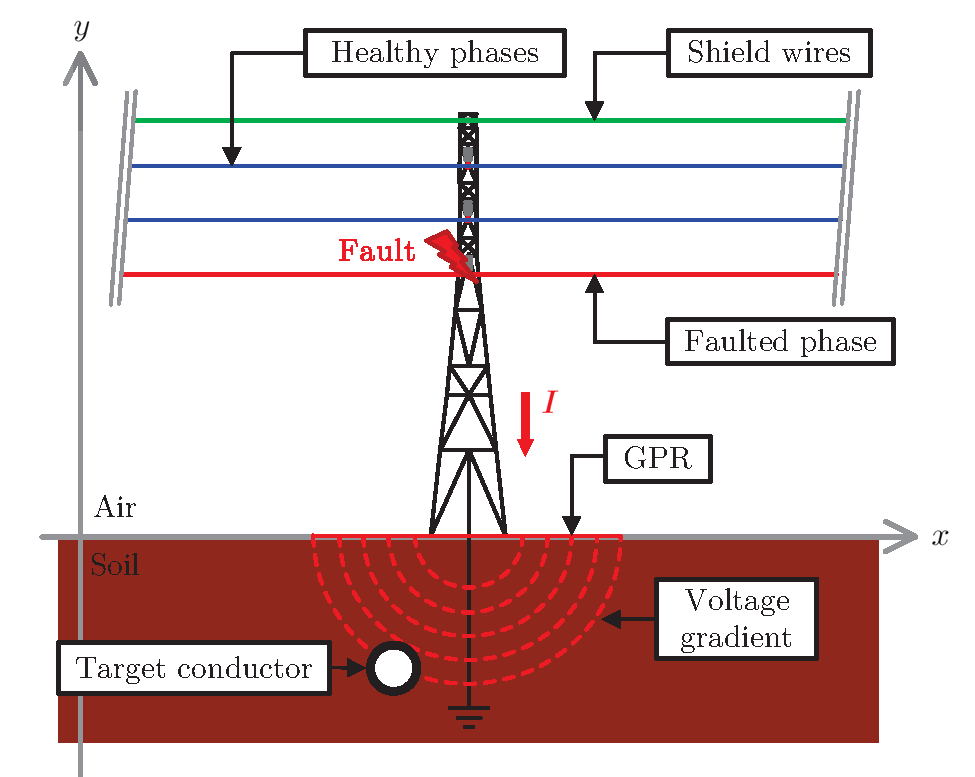
\includegraphics[width=1\columnwidth]{./fig/condu_coup2.pdf}
		\caption{Conductive coupling phenomenon, adapted from \cite{Martins-Britto2020}.}
		\label{fig:ConductiveCoupling}
	\end{center}
\end{figure} 

The current flowing into earth through the transmission line grounding conductors, also known as counterpoises, produces a GPR, which appears in the form of voltage gradients around the grounding conductors. If a target structure is within the region affected by the GPR, potentially hazardous voltages may occur.

\begin{figure*} [t]

	\begin{equation}\label{eq:Green}
		\hat{G}_{i,j}(P,O) =  \frac{1}{4\pi\hat{\sigma}_{j}} \left( \int_{0}^{\infty}A_{i,j}(\lambda)\hat{J}_{0}(\lambda r) e^{-\lambda z}d\lambda  + \int_{0}^{\infty} B_{i,j}(\lambda)\hat{J}_{0}(\lambda r) e^{\lambda z}d\lambda +  \int_{0}^{\infty} \delta(ij)\hat{J}_{0}(\lambda r) e^{-\lambda |z|}d\lambda \right)
	\end{equation}
	\hrulefill
\end{figure*}

\begin{figure}[hbt]
	\begin{center}
		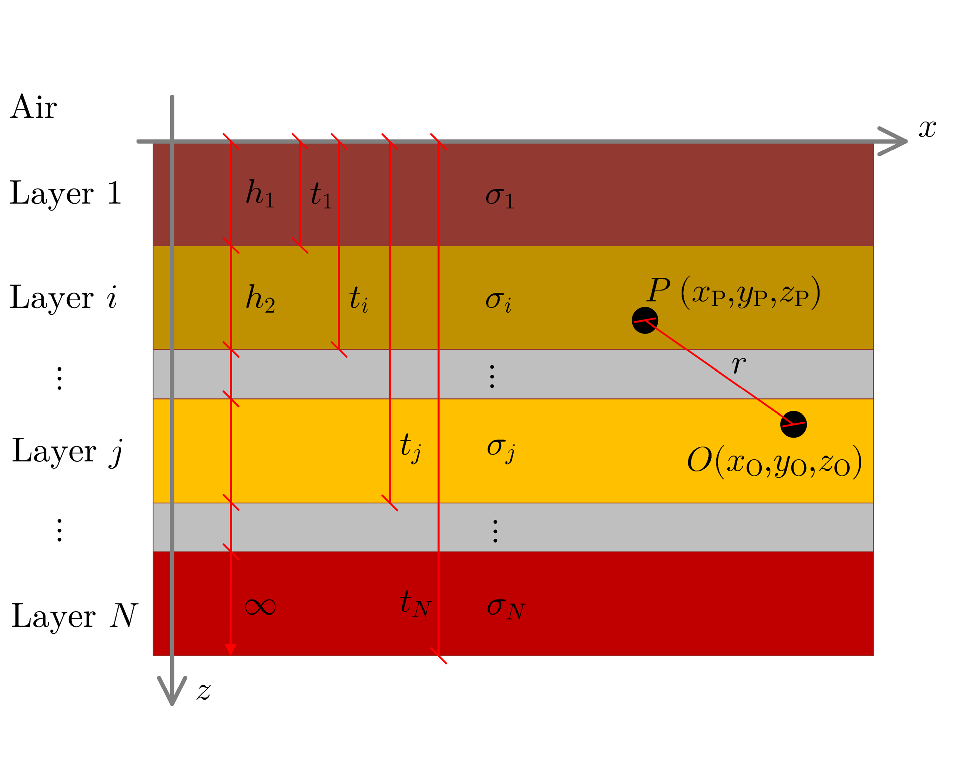
\includegraphics[width=1\columnwidth]{./fig/green_nla2.pdf}
		\caption{Point source at $i^{th}$ layer with observation point at $j^{th}$.}
		\label{fig:Greens}
	\end{center}
\end{figure}

Conductive EMI is influenced by short-circuit levels, quantity and type of shield wires, distance between the installations, grounding electrode geometry and soil properties \cite{CIGREWG36}.

In a previous work \cite{Martins-Britto2020}, the authors proposed an enhanced circuit model to account for conductive coupling in underground conductors. This approach is based on using controlled voltage sources driven by the corresponding Green's functions, as derived by He et al. \cite{He2012} and Li et al. \cite{Li2006}, which accurately express the voltage scalar potentials for N-layered media. Then, each voltage source is controlled by the currents injected into the soil by each tower within the EMI region of interest, connected to conductor coating impedance at each circuit node \cite{Martins-Britto2020}.

According to the principle of superposition, the ground potential rise $U_{P}$ at an observation point $O$, caused by the sum of all currents $I_j$ injected into the soil at each source point $P_{j}$, is given by \cite{Li2006}:

\begin{equation}
	U_{P} = \sum_{j=1}^{N} \hat{G}(P_{j},O)\cdot I_{j},
\end{equation} 

\noindent in which $U_{P}$ is the potential rise at target point $O$, in volts; $P_{j}$ are the spatial coordinates of the $j^{th}$ source point $P$; and $\hat{G}(P_{j},O)$ is a special function that describes the potential produced at point $O$ by a unit point current source located at point $P_{j}$, known as Green's function \cite{Li2006,Martins-Britto2020}.

\subsection{Green's function for N-layered soil}

The Green's function representing an earth structure with $N$ horizontal layers is developed in \cite{He2012,Li2006}. If the source point is located in the $i^{th}$ layer and the observation point is in the $j^{th}$ layer, then the Green's function general form is written as in (\ref{eq:Green}), in which $r = \sqrt{(x_{O} - x_{P})^{2} + (y_{O} - y_{P})^{2}}$ is the radius in $xy$ plane; $z = z_{O} - z_{P}$ is the vertical distance between points $O$ and $P$; $\hat\sigma_{j} = \sigma_{0} + i\omega\epsilon_{j}$ is the complex conductivity of the $j^{th}$ layer, in siemens per meter; $\hat{J}_{0}$ is the Bessel function of the first kind and order zero; and $\delta(ij)$ is the Kronecker delta, defined as equal to 1 if $i=j$ and to 0 otherwise \cite{Li2006}.

Green's function coefficients $A_{i,j}$ and $B_{i,j}$ are determined by the boundary conditions between surrounding earth layers, including the air layer above the soil surface (0-layer) and the deepest soil layer ($N$-layer), which are given as:

\begin{equation}
	\hat{G}_{i,j-1}(r,z)\vert_{z = H_{j - 1}} = \hat{G}_{i,j}(r,z)\vert_{z = H_{j-1}},
\end{equation}

\begin{equation}
	\hat\sigma_{j-1}\frac{\partial \hat{G}_{i,j-1}(r,z)}{\partial z}\bigg\vert_{z = H_{j-1}} = \hat\sigma_{j}\frac{\partial \hat{G}_{i,j}(r,z)}{\partial z}\bigg\vert_{z = H_{j-1}},
\end{equation}

\begin{equation}
	\hat{G}_{i,N}(r,z)\vert_{z\rightarrow \infty} = 0,
\end{equation}

\begin{equation}
	\frac{\partial \hat{G}_{i,0}(r,z)}{\partial z}\bigg\vert_{z\rightarrow -\infty} = 0,
\end{equation}

\noindent in which $i=1,2,\dots,N$ and $H_{0} = 0$. With the appropriate coefficients available, integrals in (\ref{eq:Green}) are solved numerically using adaptive quadratures \cite{Shampine2008}. In reference \cite{Martins-Britto2020}, Appendix A, it is provided a computer program devised to parse soil stratification data provided by the user and to compute the Green's functions values for arbitrary multilayered horizontal soils by employing the described methods. 

\subsection{Stress voltage}

An underground conductor close to a transmission line is subjected to two distinct electromagnetic effects under fault conditions, due to inductive and conductive couplings taking place simultaneously. The total voltage transferred to the interfered conductor is the potential difference between the inner metal and the external GPR, or \cite{IEEEStd80}:

\begin{equation} \label{eq:Vs}
	V_{S} = E_{T} - U_{P},
\end{equation}  

\noindent in which $V_{S}$ is the total stress voltage, in volts; $E_{T}$ is the potential of the target conductor resulting from inductive coupling, in volts; and $U_{P}$ is the local earth potential rise, in volts.

\section{Case Description}\label{sec:ScenarioDescription}

Fig. \ref{fig:Right-of-Way} illustrates a 1.2 km shared right-of-way composed by a 138 kV transmission line and an underground pipeline, in an industrial area of São Paulo, Brazil. Under nominal load conditions, the double-circuit transmission line is energized with ABC/ABC sequence, frequency 60 Hz and current of 780 A per phase. In the EMI region of interest, the transmission line is composed of 13 towers, each of which with grounding resistances of 15 $\Omega$, and two terminal substations, with grounding resistances of 1 $\Omega$. The transmission line side view and the conductor coordinates are displayed in Fig. \ref{fig:TowerGeometry}.

\begin{figure}[hbt]
	\begin{center}
		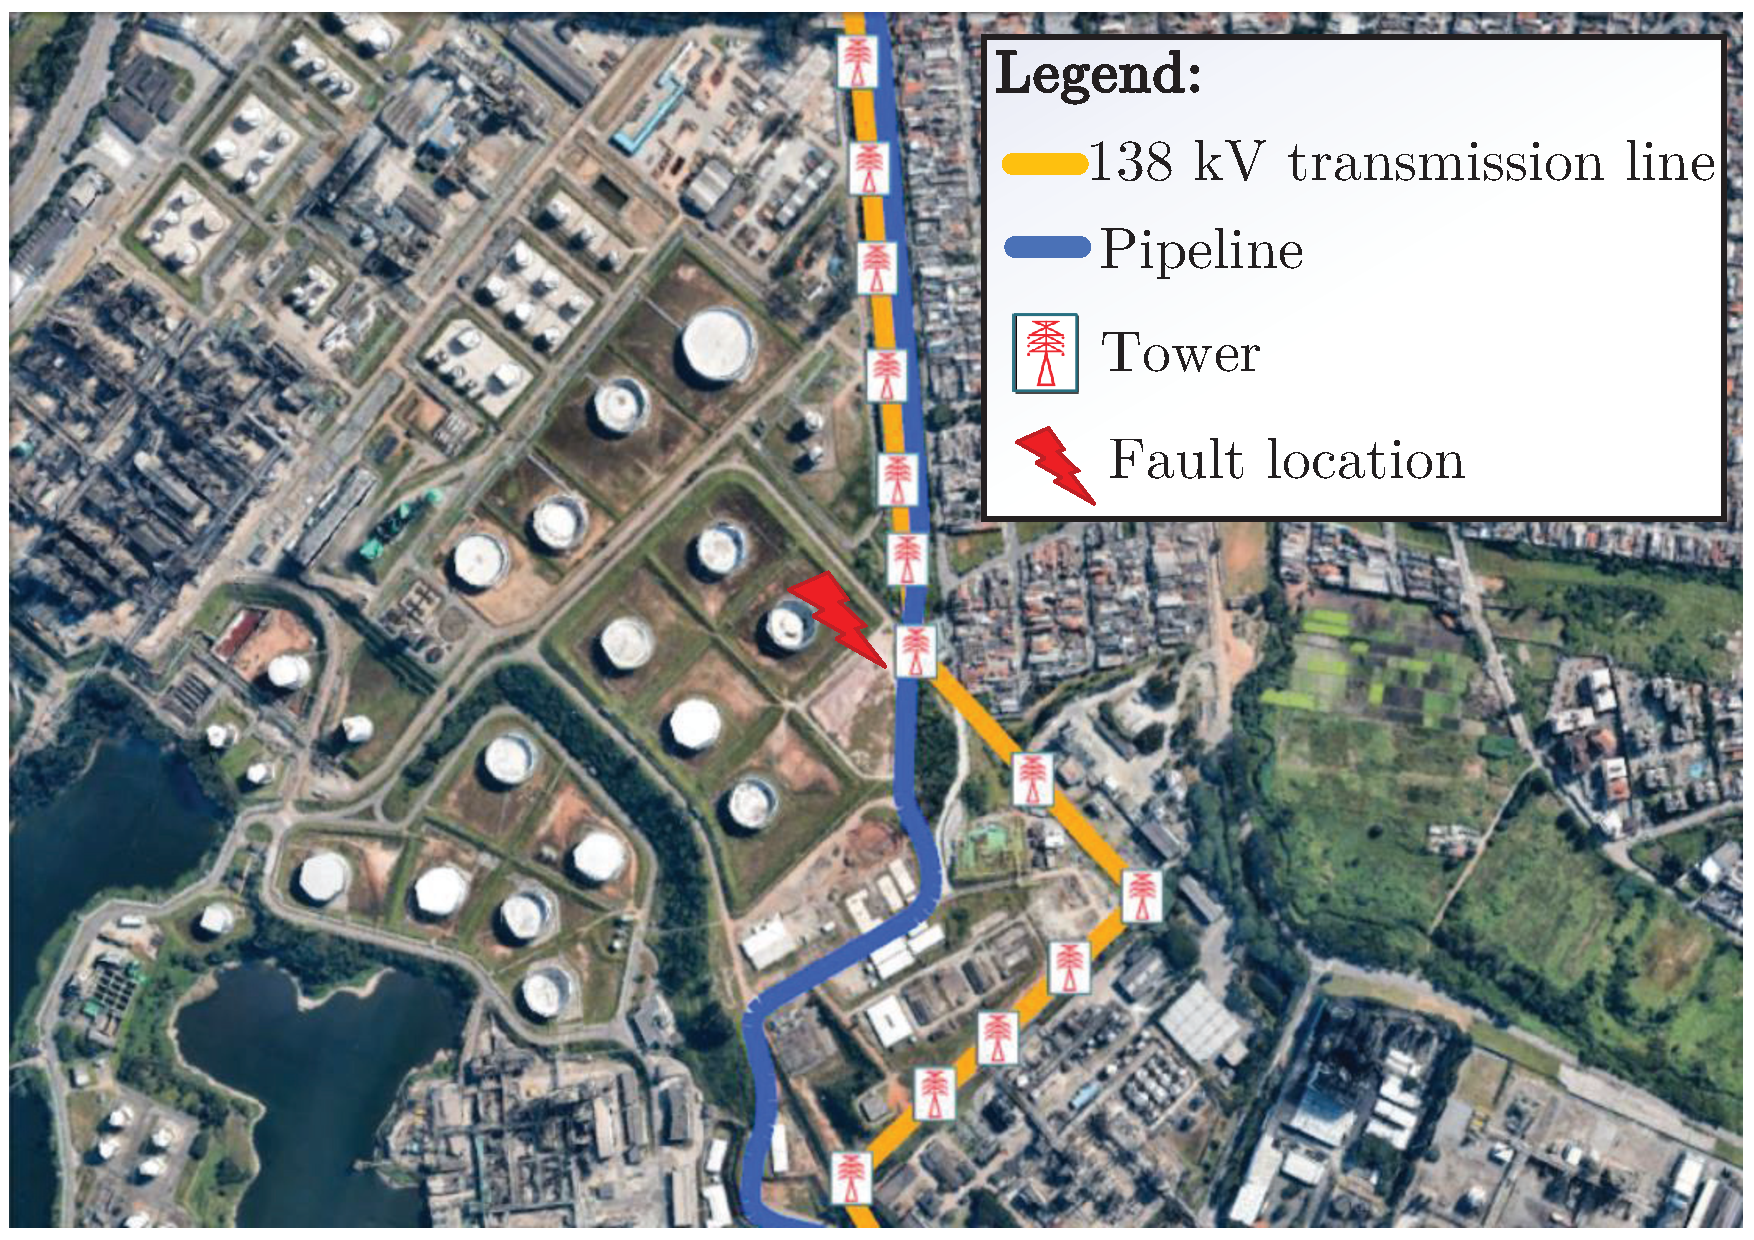
\includegraphics[width=1\columnwidth]{./fig/right-of-way2.pdf}
		\caption{Shared right-of-way between a transmission line and a pipeline in Brazil.}
		\label{fig:Right-of-Way}
	\end{center}
\end{figure}

\begin{figure}[hbt]
	\begin{center}
		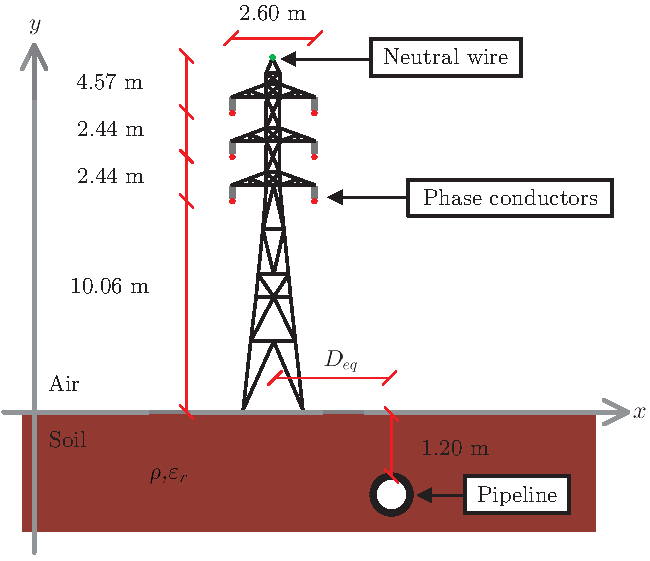
\includegraphics[width=1\columnwidth]{./fig/mutual_impedance2.pdf}
		\caption{System cross-section.}
		\label{fig:TowerGeometry}
	\end{center}
\end{figure}
 
The underground pipeline is constructed in 14" diameter carbon steel and buried 1.2 meters within the ground. The pipeline is grounded at its extremities through 10 $\Omega$ resistances. The characteristics of the transmission line conductors and the pipeline are presented in Table \ref{tab:ConductorsCharacteristics}.

\begin{table}[h]
	\renewcommand{\arraystretch}{1.3}
	\centering
	\caption{Specification and characteristics of system conductors}
	\footnotesize
	\begin{tabular}{cccc}
		\hline
		\textbf{Conductor}         & \textbf{\boldmath{$r_{out}$ [m]}} & \textbf{\boldmath{$r_{in}$ {[}m{]}}} & \textbf{\boldmath{$R_{DC}${[}$\Omega/km${]}}} \\ \hline
		{ACSR Grosbeak}     & 0.0125705                        & 0.0046355                        & 0.0924806                          \\
		{Steel 3/8" EHS-CG} & 0.004572                         & -                                & 3.42313                            \\
		{Pipe 14"}          & 0.1778                           & 0.168275                         & 0.099516                          \\ \hline
	\end{tabular}
	\label{tab:ConductorsCharacteristics}
\end{table}

The soil is modeled as a 3-layered structure based on apparent resistivity measurements performed at the right-of-way location. The specifications of the layer resistivities and thicknesses are given in Table \ref{tab:SoilParameters}.

 
\begin{table}[h]
	\renewcommand{\arraystretch}{1.3}
	\centering
	\caption{Soil parameters}
	\footnotesize
	\begin{tabular}{ccc}
		\hline
		\textbf{Layer}         & \textbf{Resistivity [\boldmath{$\Omega$}.m]} & \textbf{Thickness [m]}  \\ \hline
		1     & 488.71                        & 1.73                       \\ 
		2     & 2074.66                         & 8.99                               \\
		3     & 451.41                           & $\infty$                         \\ \hline
	\end{tabular}
	\label{tab:SoilParameters}
\end{table}

\section{Case Study Under Nominal Load Conditions}

First, a simple EMI inductive study is carried out in order to demonstrate the validity of the proposed circuit model.

\subsection{Nominal load EMTP equivalent circuit}

Due to the system geometry being composed of obliquities, crossings and parallelisms, the right-of-way is subdivided into smaller sections and, for each subdivision, it is calculated a parallel equivalent segment, as described in detail in \cite{Moraes2020}. The transmission line is modeled in the EMTP/ATP as a series of Line Constants (LCCs) objects,  which are constructed with the corresponding parallel segment parameters. Fig. \ref{fig:NLcircuit} presents the simplified circuit used for inductive simulations under nominal load conditions, in which the objects labeled as TACS are the controled voltage sources native of ATP, representing the sum of the EMFs produced by phase conductors and shield wires. The current probes of the TACS sources are placed to measure the series current at each LCC output terminal and the current values are used to build the EMF sources distributed along the interfered conductor, represented in the inferior part of Fig. \ref{fig:NLcircuit}.

\begin{figure}[hbt]
	\begin{center}
		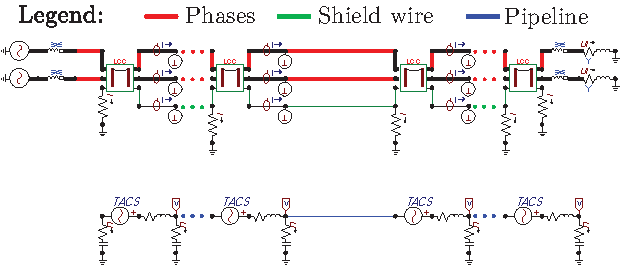
\includegraphics[width=1\columnwidth]{./fig/NL_circuit2.pdf}
		\caption{Nominal load EMTP simplified model representation.}
		\label{fig:NLcircuit}
	\end{center}
\end{figure}

\subsection{Nominal load simulation results}

Fig. \ref{fig:NLvoltage} shows the induced voltage along the pipeline using the proposed model, as well as the comparison with the EMI reference software CDEGS \cite{Dawalibi1984a}. 

\begin{figure}[hbt]
	\begin{center}
		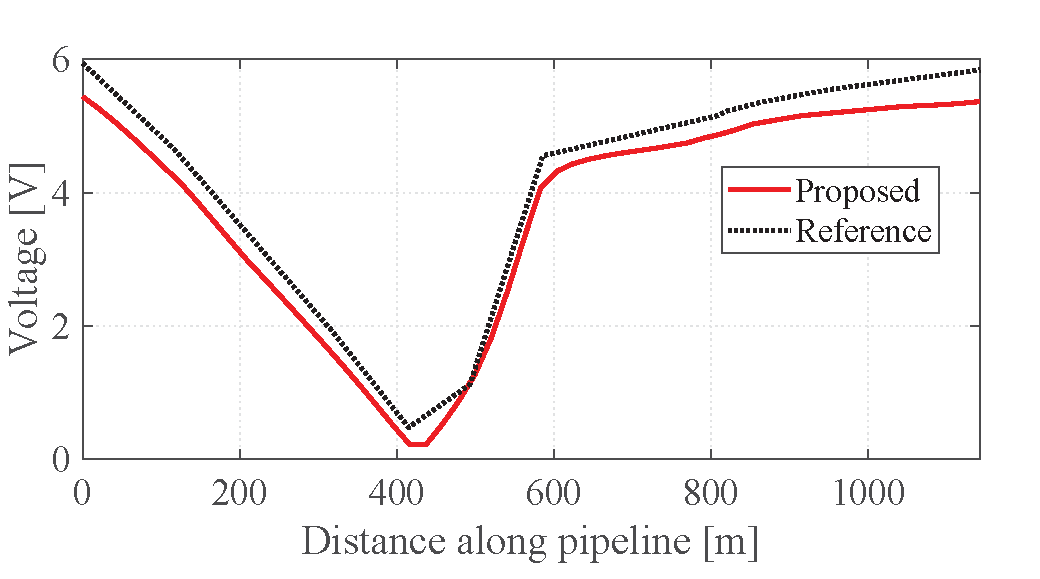
\includegraphics[width=1\columnwidth]{./fig/NL_voltage2.pdf}
		\caption{Induced voltage along the pipeline under nominal load conditions.}
		\label{fig:NLvoltage}
	\end{center}
\end{figure}

Results show that the proposed model agrees with the reference software, presenting an RMS error of 7.35\%, which is
mainly explained by the different line models and impedance formulations used in each approach.

Due to the grounding resistance at the pipeline extremities, the induced voltage does not exceed the safety limit of 15 V in steady-state regime \cite{NACEInternational2007}. Grounding resistances provide a safe path to the induced currents flow back into the earth, thus preventing risks to the interfered installation. 

As the proposed circuit model is considered to be validated, the next section follows with the simulation of a more complex scenario, consisting of a possible fault situation and its impacts on the nearby pipeline.

\section{Case Study Under Fault Conditions}

In order to study the ground potential rise and the total stress voltage, a phase-to-ground fault is applied to the system presented in Section \ref{sec:ScenarioDescription}.

\subsection{Fault regime EMTP equivalent circuit}

The phase-to-ground fault is assumed to occur at tower \#7. A resistance value of 0.001 $\Omega$  is chosen to represent a short-circuit between the phase B conductor and the shield wire.

\begin{figure}[hbt]
	\begin{center}
		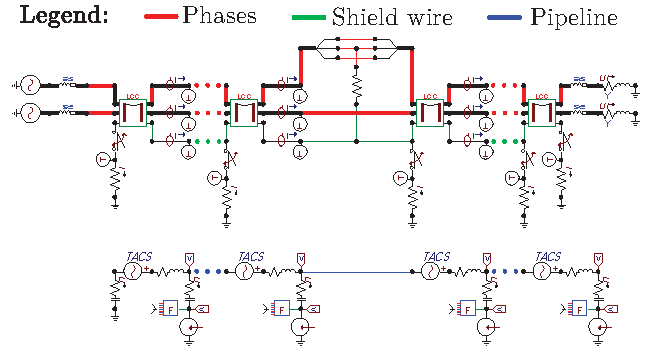
\includegraphics[width=1\columnwidth]{./fig/Fault_circuit2.pdf}
		\caption{EMTP simplified model representation for fault regime study.}
		\label{fig:FaultCircuit}
	\end{center}
\end{figure}

Fig. \ref{fig:FaultCircuit} shows the simplified equivalent circuit for fault simulations. The model is constructed by following the same procedure described in the preceding section. However, additional TACS sources are connected to the pipeline coating impedance to represent the ground potential rise due to conductive coupling. The current probe of the TACS sources measures the current flowing through each tower grounding impedance to the local earth.

\subsection{Fault condition simulation results}

The potential resulting from inductive coupling, the local ground potential rise and the resulting stress voltage distribution due to the phase-to-ground fault simulated are presented in Fig. \ref{fig:Faultvoltage}.

\begin{figure}[hbt]
	\begin{center}
		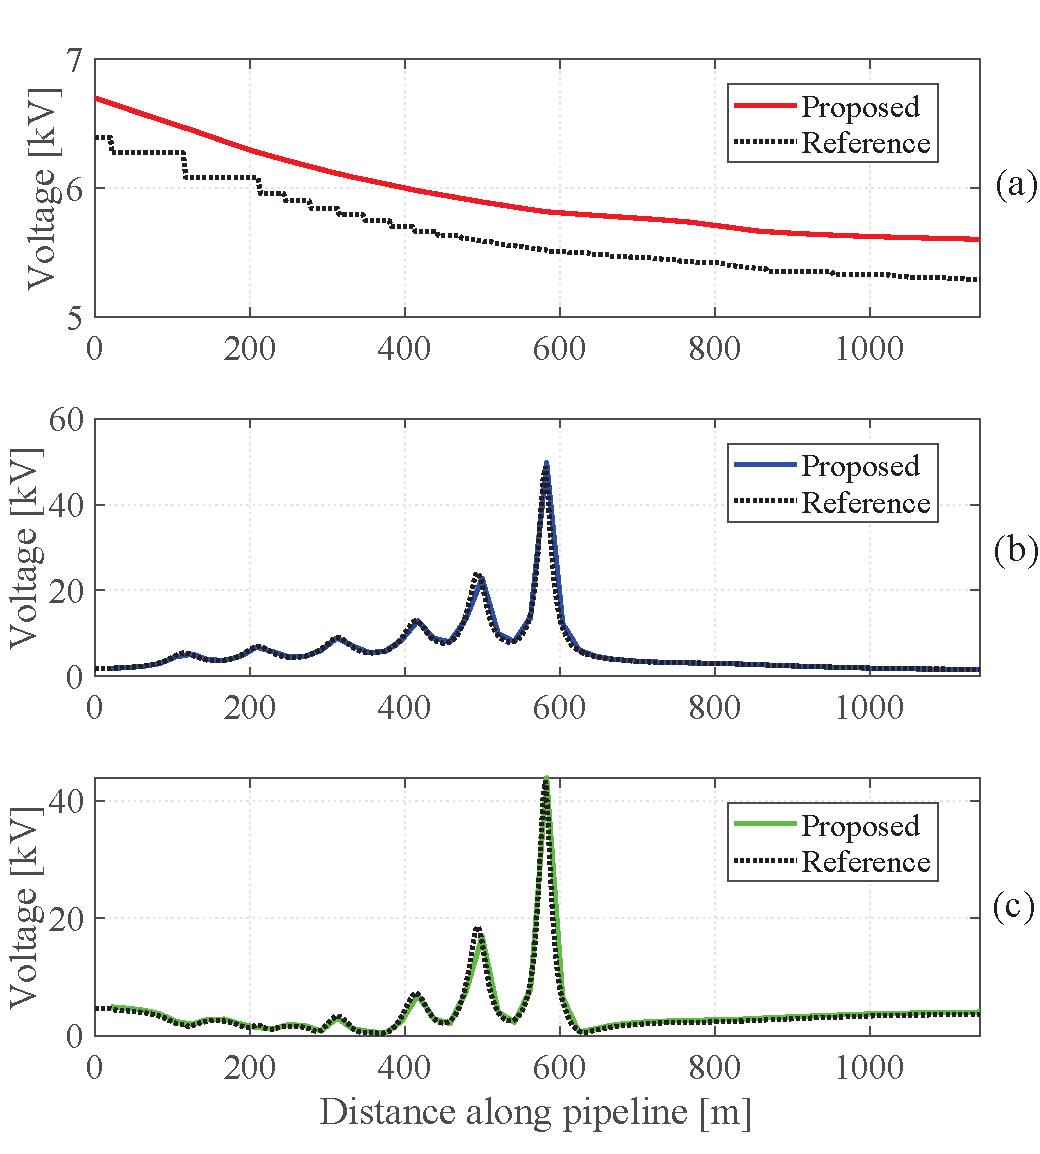
\includegraphics[width=1\columnwidth]{./fig/Fault_voltage2.pdf}
		\caption{Pipeline voltage due to: (a) inductive coupling; (b) GPR; and (c) total stress.}
		\label{fig:Faultvoltage}
	\end{center}
\end{figure}

The obtained results agree with the reference software, with RMS errors of 1.42\% and 1.21\%, respectively. The inductive  voltage presented a RMS error of 21.17\%. However, since both curves present the same shape with a nearly constant offset, it is relevant to observe also the average relative error. In this case, the inductive coupling voltage presents a deviation of 5.5\%.

The total stress voltage along the pipeline reaches 43.9 kV close to the fault location, which may cause dielectric breakdown of the coating layer, exposing the metal to electrochemical corrosion \cite{NACEInternational2007}. Modern pipeline coating materials, such as the 3-Layer Polyethylene (3LPE), are designed to withstand voltages up to 25 kV, according to manufacturer's information \cite{NACEInternational2007}.

Fig. \ref{fig:Faultcurrent} shows the currents flowing in the shield wires and through the tower groundings. The largest values occur in the vicinities of the faulted tower, which justifies the shape of the GPR curve shown in Fig.\ref{fig:Faultvoltage}-b.   

\begin{figure}[hbt]
	\begin{center}
		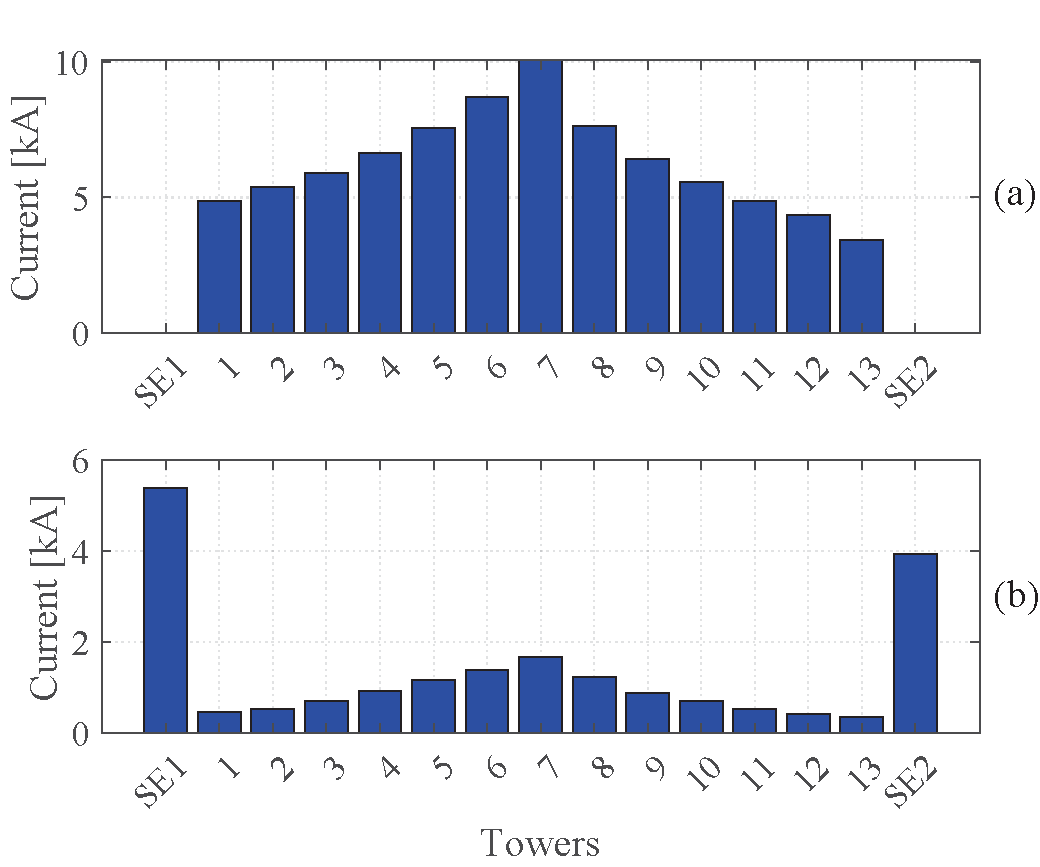
\includegraphics[width=1\columnwidth]{./fig/Fault_current2.pdf}
		\caption{(a) Ground currents; and (b) currents flowing through the shield wire.}
		\label{fig:Faultcurrent}
	\end{center}
\end{figure}

\section{Mitigation Study}

As the total stress under fault conditions far exceeds safety limits, which may present risks to the pipeline integrity, a mitigation design is proposed. The proposed mitigation consists of connecting the pipeline to the earth at regularly-spaced points using an adequately sized grounding conductor ($\leq 10$ $\Omega$). This method is used to transfer the external ground potential rise to the inner metal, thus reducing the difference in (\ref{eq:Vs}) and, consequently, decreasing the resulting stress voltages. 

In the case shown in this paper, the hazardous region is located from 450 to 650 meters along the pipeline path. Within this zone, the pipeline is grounded at every 40 m through 1 $\Omega$ resistors. Fig. \ref{fig:Mitvoltage} presents the comparison between the pipeline voltages before and after the mitigation.    

\begin{figure}[hbt]
	\begin{center}
		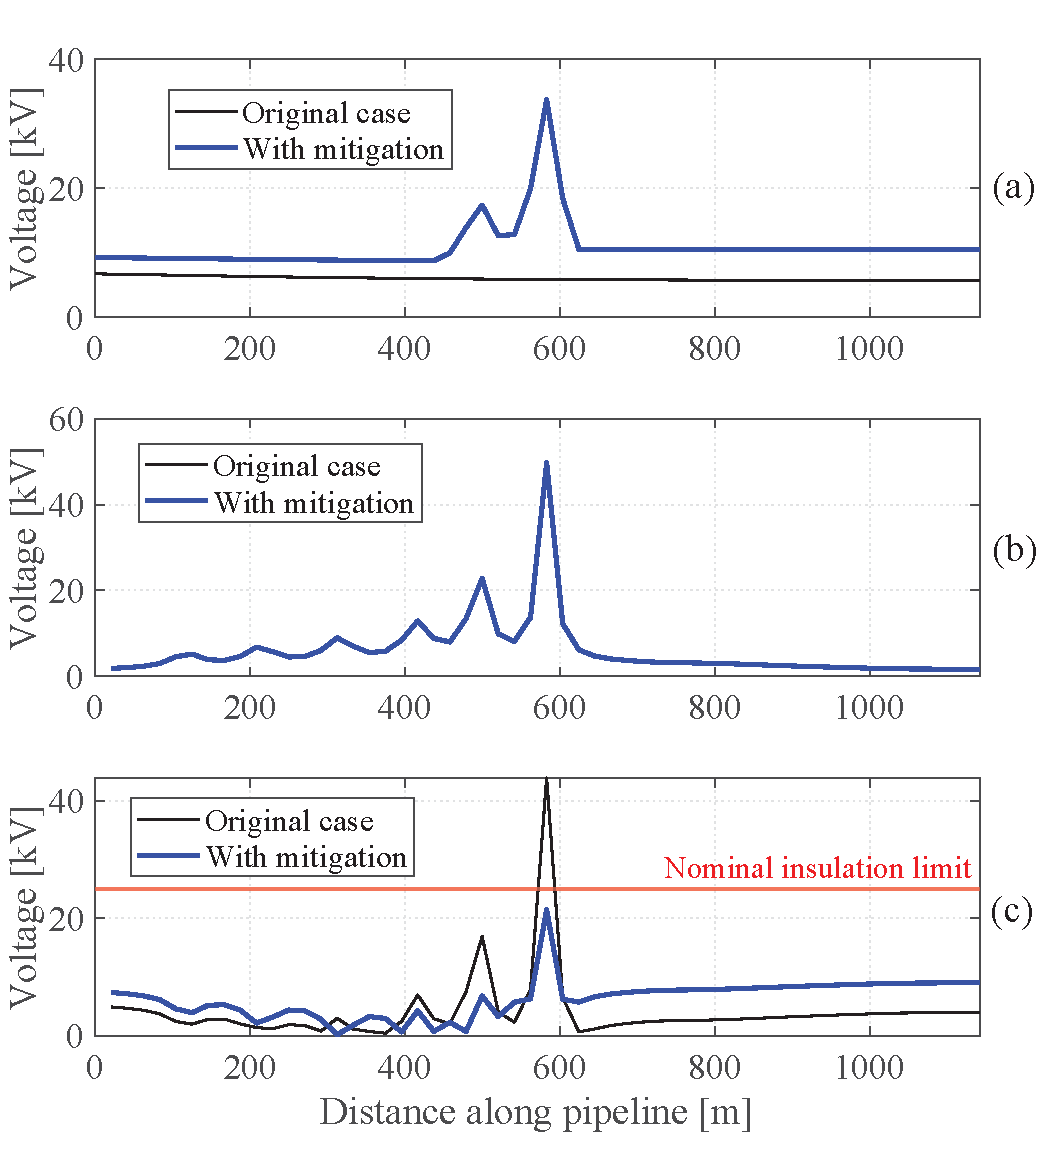
\includegraphics[width=1\columnwidth]{./fig/Mit_voltage2.pdf}
		\caption{Comparison of pipeline voltages before and after the mitigation due to: (a) inductive coupling; (b) GPR; and (c) total stress.}
		\label{fig:Mitvoltage}
	\end{center}
\end{figure}

Is observed that the proposed mitigation design reduces the maximum stress voltage to 21 kV, thus meeting the safety criteria adopted in pipeline industry \cite{NACEInternational2007}. 

It is important to notice that the mitigation method is efficient to reduce the stress voltages in the intended location. However, for regions outside the mitigation influence, the pipeline potential may rise. This is related to the inner pipeline voltage reaching 33 kV, approximately 6.6 times superior to the original case, which is exactly the equipotential condition sought in grounding designs.

\section{Conclusions}

This work presented an EMTP-based circuit approach to predict total stress voltages in a pipeline due to a transmission line phase-to-ground faults. The proposed method is based on formulations which effectively represent multilayered soils without approximations or uniform equivalents. 

To validate the proposed methodology, a real case of right-of-way shared between an underground pipeline and a double-circuit 138 kV transmission line was modeled and tested, under nominal and fault conditions. 

Results showed that the methodology is valid and accurate under both nominal and fault condition scenarios, presenting a maximum error of 7.35\% in comparison with  EMI analysis industry-standard software.

Under nominal conditions, the maximum induced voltage reached 6 V, being considered a safe value to the facilities and personnel involved. However, under phase-to-ground fault conditions, the stress voltage reached almost 44 kV, which may be hazardous for the pipeline coating and without conformity with the nominal limits established for the industry. 

For this reason, further studies were carried out and a mitigation was designed to handle the case under study. The method consisted of grounding the pipeline along the hazardous zone. The results obtained proved that the mitigation method is efficient, having decreased  the original voltages in 47\%, leading the final stress to below the 25 kV safe limit. 

This work offered relevant insights of how resourceful the EMTP-based EMI simulation techniques can be when applied to problems of practical relevance to the industry, especially when one is concerned with the safety of facilities and personnel involved.

\bibliographystyle{IEEEtran}
\nocite{*}
\bibliography{refs}

\end{document}


